\chapter[Results and Discussions]{Results and Discussions}{Results and Discussions}\label{res}
The findings indicate the realistic application of the TrustChain model as a working web based decentralized identity verification system. The interfaces put in place en-sure validation of controlled access, privacy preserving verification and on-chain auditability of actual user and institutional interactions. The dashboard enables registered institutions to find individuals and make credential access requests. The organization will be able to seek verification without looking at the raw identity documents, which will enforce a least privilege access rule. This screen is used to capture the user approving the access by providing the credential hash only. Authentication of identity is done by cryptographic validation, and not by document disclosure. Successful verification is displayed in this interface in which access is granted and validated. The institution is presented with proof of originality without the access to personal identity information. This is the last perspective in which institutions can check the verification status of an individual. The outcome warrants identity validity and privacy and continues access control that is revocable. This illustrates the usefulness of a proof based verification model in the real world. The system is able to remove needless data exposure and at the same time retain trust between entities. It also emphasizes the role of user controlled consent in the process of identity sharing. The findings verify that decentralized strategies may be beneficial in terms of security and transparency. This enhances the possibility of integration with the current digital identity ecosystems. TrustChain is an overall viable and scalable solution to privacy oriented identity verification.

\section{Outputs}
\begin{figure}[h!]
    \centering
    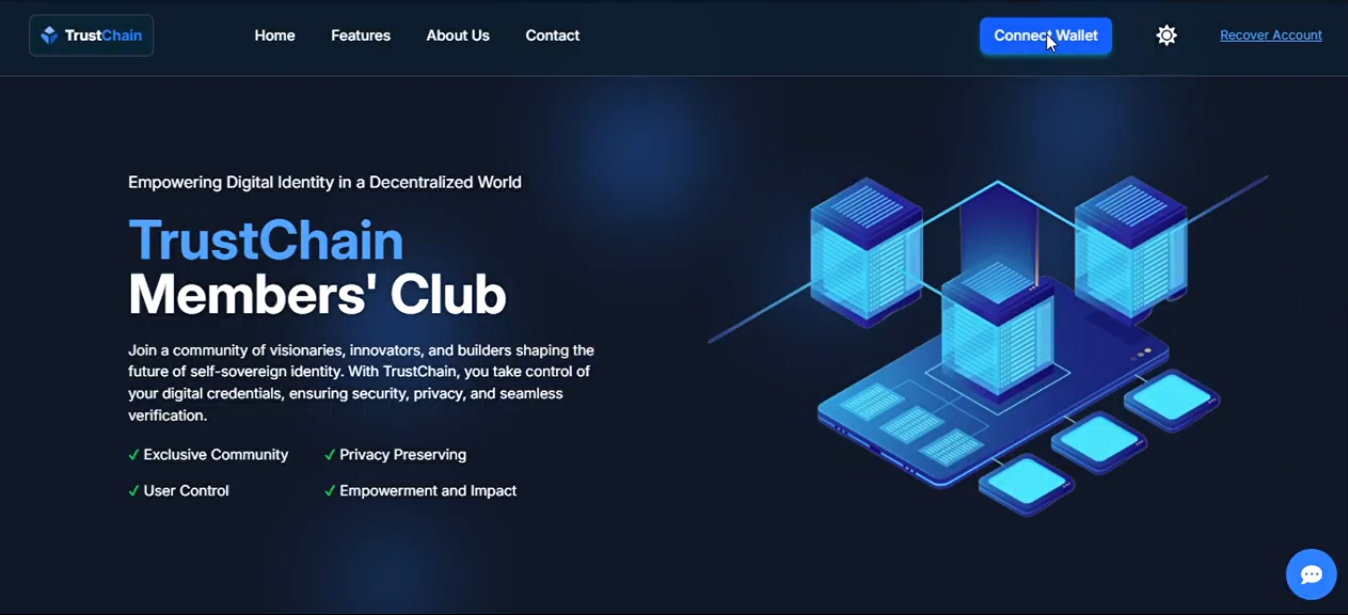
\includegraphics[width=0.8\textwidth]{Chapter1/dashboard.png} % Adjust the width as needed
    \caption{TrustChain Dashboard}
    \label{f1} % Optional: for referencing the figure in your document
\end{figure}

\begin{figure}[h!]
    \centering
    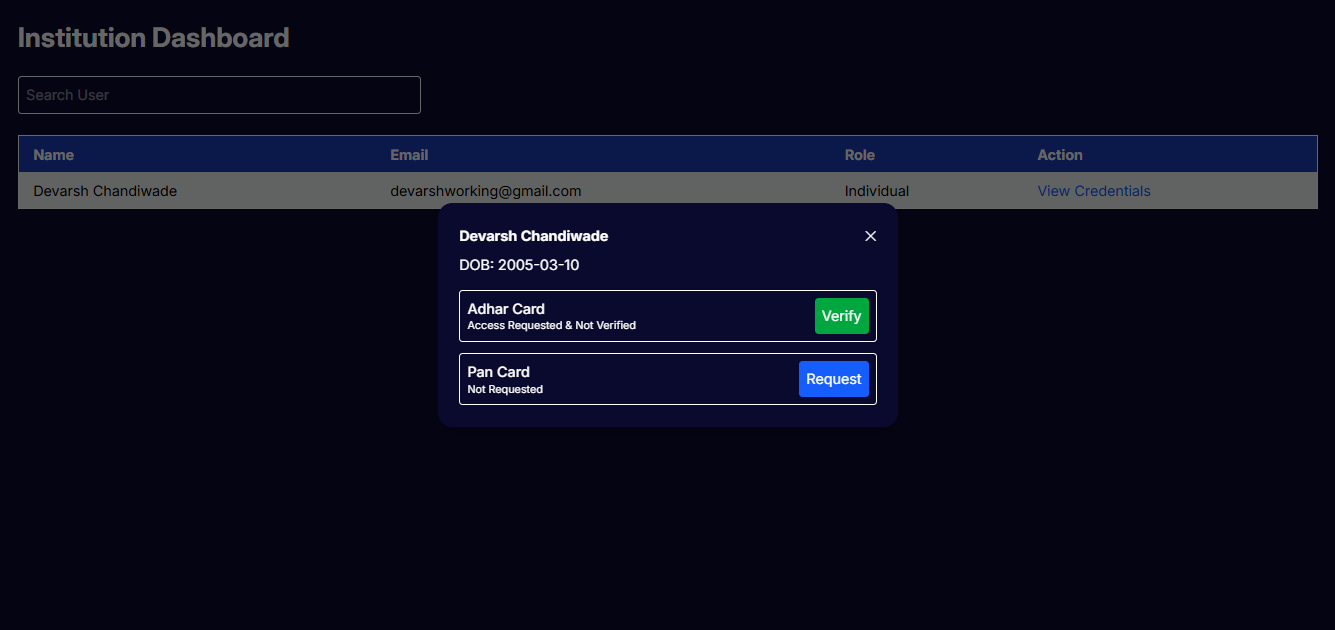
\includegraphics[width=0.8\textwidth]{Chapter1/ss2.png} % Adjust the width as needed
    \caption{Institution Dashboard for Credential Request}
    \label{f1} % Optional: for referencing the figure in your document
\end{figure}

\begin{figure}[h!]
    \centering
    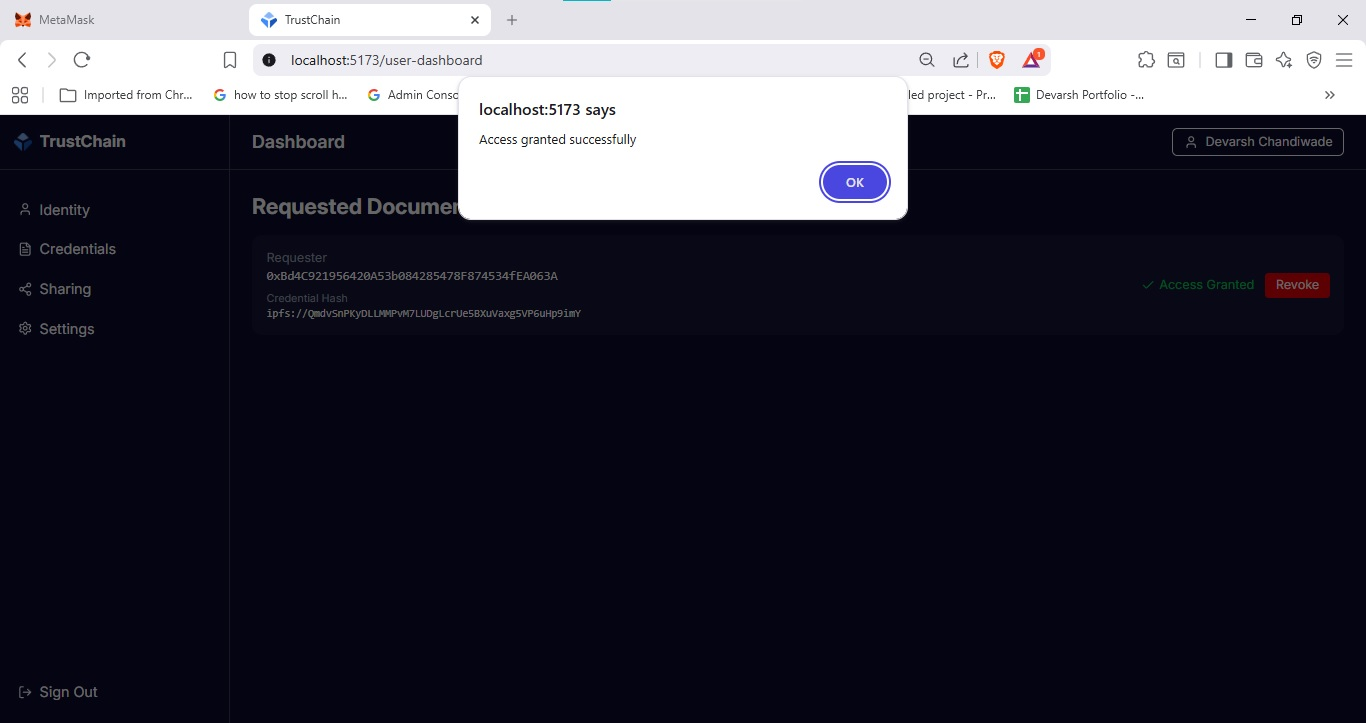
\includegraphics[width=0.8\textwidth]{Chapter1/ss4.jpeg} % Adjust the width as needed
    \caption{Individual Granting Credential Hash Access}
    \label{f1} % Optional: for referencing the figure in your document
\end{figure}

\begin{figure}[h!]
    \centering
    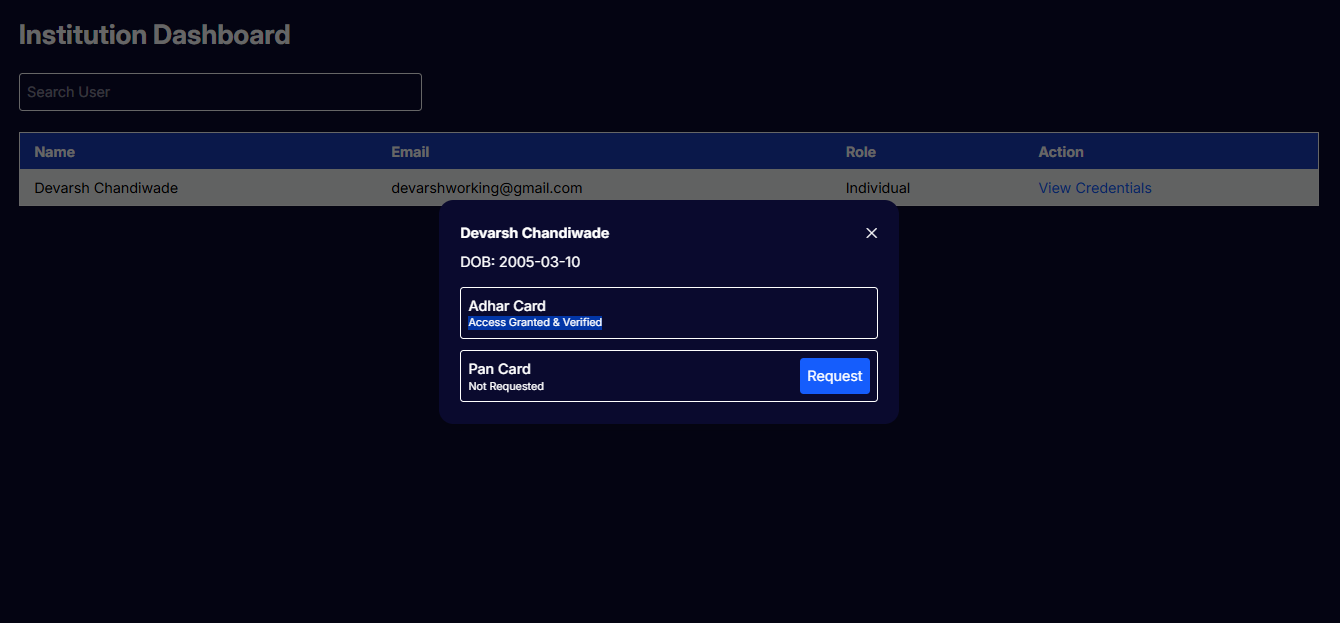
\includegraphics[width=0.8\textwidth]{Chapter1/ss5.png} % Adjust the width as needed
    \caption{Institution Verification Confirmation View}
    \label{f1} % Optional: for referencing the figure in your document
\end{figure}

\begin{figure}[h!]
    \centering
    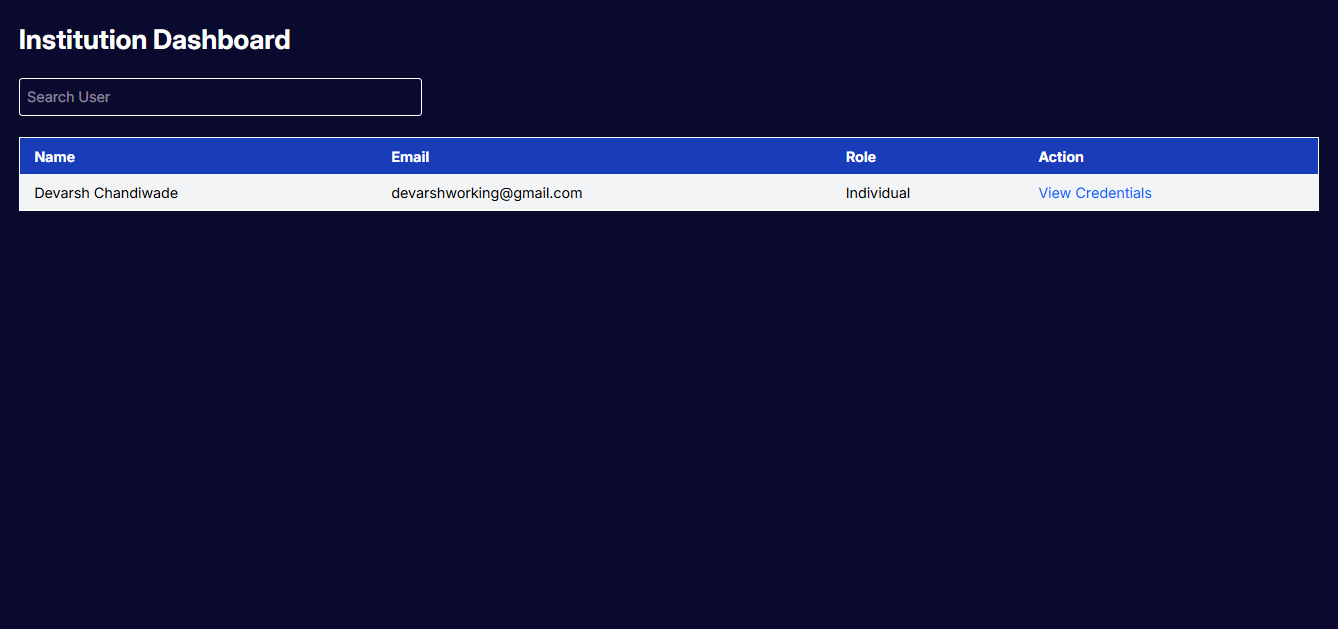
\includegraphics[width=0.8\textwidth]{Chapter1/ss6.png} % Adjust the width as needed
    \caption{Institution View of Verified Identity Status}
    \label{f1} % Optional: for referencing the figure in your document
\end{figure}


\chapter{Conclusions \& Future Scope}
